%\makeatletter
%\def\toclevel@chapter{0}
%\makeatother


\chapter{Approche spectrale}
%\begin{tikzpicture}[remember picture, overlay]
%\node[anchor=north east,inner sep=0pt] at (current page.north east) {
\includegraphics[scale=1]{Fig/Chapter1/g825.png}};
%\end{tikzpicture}
\label{ch:TauS_NJP}

Dans le chapitre précédent, nous nous sommes concentrés sur la mesure du temps de diffusion élastique, que nous avons comparé à la théorie perturbative de Born. En particulier, nous avons montré que celle-ci fournit une prédiction quantitative du temps de diffusion élastique dans le régime de diffusion faible, mais que de fortes déviations apparaissent lorsque l'amplitude du désordre $|\VR|$ augmente et que l'impulsion initiale $k_{\mathrm{i}}$ diminue. La comparaison de nos données à la prédiction de Born nous a de plus permit d'étudier quantitativement la transition entre les régimes de diffusion faible et diffusion forte, révélant ainsi la forte influence de la distribution du potentiel sur la position de cette transition \citep{richard2019elastic}. 

Néanmoins, l'approximation de Born échoue à décrire le régime de diffusion forte. Dans ce chapitre, nous décrirons le comportement du temps de diffusion élastique à l'aide des fonctions spectrales mentionnées au chapitre \ref{ch:Localisation} et au formalisme de la fonction de Green. Plus particulièrement, nous estimerons les fonctions spectrales à l'aide du développement de Born et à l'aide d'une approche auto-consistante. Enfin, nous comparerons nos valeurs expérimentales du temps de diffusion élastique à des valeurs extraites de la mesure expérimentales des fonctions spectrales.

L'étude présentée ici a fait l'objet d'une publication dans la revue \emph{New Journal of Physics} \citep{signoles2019ultracold}.

\section{Temps de diffusion élastique et fonctions spectrales}

Dans un premier temps, nous allons présenter le lien entre le temps de diffusion élastique $\taus(\VR,\mathbf{k}_{\mathrm{i}})$ et la fonction spectrale $A(\mathbf{k}_{\mathrm{i}},E)$. Nous décrirons ensuite les approximations couramment utilisées pour la détermination de cette dernière, dont nous allons extraire un temps de vie $\taus^{\mathrm{sf}}$ que nous confronterons à nos mesures. 


\subsection{Généralités sur la fonction spectrale}
Le hamiltonien $\hat{H}$ d'une particule quantique soumise à un potentiel peut être décomposé sous la forme
\begin{equation}
\hat{H}=\hat{H}_0+\hat{V} \text{ ,}
\end{equation}
avec $\hat{H}_0$ le hamiltonien non perturbé, dont nous supposerons connaître les états propres, et $\hat{V}$ le potentiel venant perturber la particule. Dans le cadre de la propagation d'ondes dans un milieu désordonné, nous pouvons identifier $\hat{H}_0$ à l'énergie cinétique $\hat{p}^2/2m$ dont les états propres correspondent aux ondes planes $\lbrace \etat{\mathbf{k}} \rbrace$ et $\hat{V}$ au désordre ressenti par les atomes.

\paragraph*{Fonction de Green}
Un outil couramment utilisé pour décrire l'évolution de ce système quantique est la fonction de Green, qui correspond à la réponse impulsionnelle de l'équation de Schrödinger. La fonction de Green peut s'écrire
\begin{equation}
\hat{G}(E)=\frac{1}{E-\hat{H}+i 0^+} 
\label{eq:definition_green}
\end{equation}
dans la base des énergies \citep{akkermans2007mesoscopic}\citep{kuhn2007coherent}. En remplaçant le hamiltonien $\hat{H}$ par son expression, on montre ainsi que la fonction de Green est solution de l'équation de Dyson
\begin{equation}
\hat{G}(E)=\hat{G}_0(E) + \hat{G}_0(E) \hat{V} \hat{G}(E) \text{ ,}
\label{eq:dyson}
\end{equation}
où $\hat{G}_0(E)$ est la \emph{fonction de Green libre}, qui correspond à la fonction de Green en absence de désordre, régissant donc la dynamique des ondes planes $\lbrace\etat{\mathbf{k}}\rbrace$ états propres du hamiltonien non perturbé $\hat{H}_0$. Exprimée dans la base des ondes planes où la fonction de Green libre est diagonale, celle-ci s'écrit 
\begin{equation}
G_0(E,\mathbf{k}_{\mathrm{i}})=\left\langle\mathbf{k}_{\mathrm{i}} | \hat{G}_0(E)| \mathbf{k}_{\mathrm{i}} \right\rangle =\frac{1}{E-E_{\mathrm{k}_i}+i0^+} \text{ ,}
\end{equation}
avec $E_{\mathrm{k}_i}$ l'énergie cinétique de la particule. 

À l'aide de l'équation de Dyson \ref{eq:dyson}, on peut déterminer la fonction de Green moyenne 
\begin{equation}
\overline{G}(E,\mathbf{k}_{\mathrm{i}})=\frac{1}{E-E_{\mathrm{k}_i}-\overline{V}-\Sigma(E,\mathbf{k}_{\mathrm{i}})} \text{ ,}
\label{eq:fonction_green_moyenne}
\end{equation}
où $\overline{\cdots}$ représente la moyenne sur les différentes réalisations du désordre. La quantité complexe $\Sigma(E,\mathbf{k}_{\mathrm{i}})$, la \emph{Self-Energy}, est homogène à une énergie et encode l'effet des fluctuations du potentiel désordonné $\hat{V}$\footnote{Seules les fluctuations du potentiel sont contenues dans la self-energy telle qu'écrite ici puisque nous avons fait apparaître explicitement la valeur moyenne du potentiel.}. Si l'expression de la fonction de Green moyenne \ref{eq:fonction_green_moyenne} est exacte, sa détermination reste ardue et demande l'utilisation d'approximations pour déterminer la self-energy, telles que l'expansion de Born\citep{kuhn2007coherent}\citep{lugan2009one}, l'approche auto-consistante de Born \citep{skipetrov2008anderson}\citep{yedjour2010diffusion}, ou encore des approximations semi-classiques \citep{trappe2015semiclassical}\citep{prat2016semiclassical}. 


\paragraph*{La fonction spectrale}
La fonction spectrale est définie à l'aide de la fonction de Green moyenne par
\begin{equation}
A(\mathbf{k}_{\mathrm{i}},E)= -\frac{1}{\pi} \mathrm{Im}[\overline{G}(E,\mathbf{k}_{\mathrm{i}})] \text{ .}
\end{equation}
Le calcul des fonctions spectrales, essentielle à la bonne description de la dynamique de l'onde dans le désordre (voir section \ref{sc:etat_art_transition}), repose donc directement sur la détermination de la fonction de Green moyenne.

Étant donné que la fonction de Green moyenne est entièrement déterminée par la self-energy, il est aussi possible d'exprimer la fonction spectrale à l'aide de la self-energy:
\begin{equation}
A(\mathbf{k}_{\mathrm{i}},E)=-\frac{1}{\pi}\frac{\mathrm{Im}[\Sigma(E,\mathbf{k}_{\mathrm{i}})]}{(E-E_{\mathrm{k},i}-\overline{V}-\mathrm{Re}[\Sigma(E,\mathbf{k}_{\mathrm{i}})])^2+\mathrm{Im}[\Sigma(E,\mathbf{k}_{\mathrm{i}})]^2} \text{ .}
\label{eq:fonction_spectrale_self_energy}
\end{equation}
Un intérêt particulier de cette expression est de fournir une idée intuitive de la forme de la fonction spectrale dans les différents régimes de diffusion, résumés figure \ref{fig:illustration_fonction_spectrale_diffusion}. 

En effet, il est possible de montrer que dans la limite des désordres très faibles, la self-energy varie très lentement autour de l'énergie cinétique $E_{\mathrm{k}_i}$ \citep{kuhn2007coherent}. La forme de la fonction spectrale sera donc très proche d'une lorentzienne, dont le centre est déplacé par la valeur moyenne du potentiel et la partie réelle de la self-energy, et de largeur liée à la partie imaginaire de la self-energy\footnote{Dans le cas d'une particule libre, la fonction spectrale est donnée par une distribution de Dirac centrée sur l'énergie cinétique $A(\mathbf{k}_{\mathrm{i}},E)=\delta(E-\Eki)$. On retrouve la relation de dispersion d'une particule libre.}, comme illustré figure \ref{fig:illustration_fonction_spectrale_diffusion}.a. 


Il est aussi possible de deviner la forme de la fonction spectrale dans la limite de désordres très forts $|\VR|\gg\ER$, c'est à dire dans la limite de désordres classiques. Dans ce régime, la fonction spectrale, qui est la probabilité qu'une particule d'impulsion $\mathbf{k}_{\mathrm{i}}$ ait une énergie $E$, converge vers la distribution du potentiel. En effet dans cette limite classique aussi notée $\hb\rightarrow 0$, l'énergie de la particule est la somme de l'énergie cinétique $\Eki$ et de l'énergie potentielle $V$. La probabilité d'avoir une énergie $E$ est donc simplement donnée par la probabilité d'avoir une énergie potentielle $V$, c'est à dire $\mathcal{P}(V)$. Dans cette limite, la fonction spectrale est donc donnée par \citep{trappe2015semiclassical}
\begin{equation}
A^{\mathrm{cl}}(\mathbf{k}_{\mathrm{i}},E)\approx \mathcal{P}(E-\Eki) \text{ ,}
\end{equation}
comme représenté dans le dernier cadre de la figure \ref{fig:illustration_fonction_spectrale_diffusion}. 


\begin{figure}
\centering
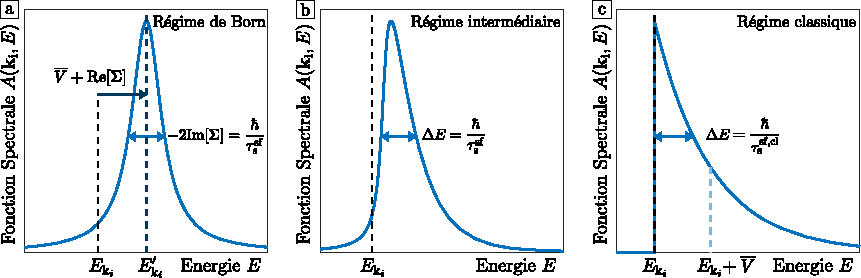
\includegraphics[width=\textwidth]{Fig/TauS_NJP/illustration_fonction_spectrale_diffusion.pdf}
\caption{\textbf{Illustration du profil de la fonction spectrale dans les différents régimes de diffusion.} \textbf{a.} Dans la limite d'un désordre faible, la self-energy est approximativement constante autour de l'énergie cinétique. La forme de la fonction spectrale est alors lorentzienne, dont la largeur est donnée par la partie imaginaire de la self-energy, inversement proportionnelle au temps de diffusion élastique $\taus^{\mathrm{sf}}$. \textbf{b.} Fonction spectrale dans le régime intermédiaire, pour lequel aucune prédiction générale n'existe. On peut néanmoins définir un temps de diffusion élastique effectif $\taus^{\mathrm{sf}}$ à l'aide de la largeur de la fonction spectrale. \textbf{c.} Dans la limite classique d'un désordre très fort, la fonction spectrale converge vers la distribution de potentiel décalée de l'énergie cinétique initiale. Cette situation est illustrée ici pour un speckle répulsif.}
\label{fig:illustration_fonction_spectrale_diffusion}
\end{figure}


\paragraph*{Lien entre la fonction spectrale et la décroissance de l'état initial}
Il est possible de déterminer d'autres expressions de la fonction spectrale en revenant à la définition de la fonction de Green \ref{eq:definition_green}. Notamment, on peut montrer que
\begin{equation}
A(\mathbf{k}_{\mathrm{i}},E)=-\frac{1}{\pi} \overline{\langle \mathbf{k}_{\mathrm{i}} | \mathrm{Im}\left[G(E)\right]| \mathbf{k}_{\mathrm{i}} \rangle} = \overline{\langle \mathbf{k}_{\mathrm{i}} | \delta(E-\hat{H})|\mathbf{k}_{\mathrm{i}}\rangle} \text{ ,}
\end{equation}
en utilisant la relation $ 1/(x+i0^+)=\mathrm{vp}(1/x)-i\pi \delta(x)$. 

En utilisant la représentation exponentielle de la distribution de Dirac, on peut alors montrer que l'opérateur évolution moyen $\overline{U}_{\mathrm{k}_i}$ de l'état initial est simplement donné par la transformée de Fourier de la fonction spectrale
\begin{equation}
\overline{U}_{\mathrm{k}_{\mathrm{i}}}(t)=\left\langle \mathbf{k}_{\mathrm{i}} | \overline{\exp(-itH)}  | \mathbf{k}_{\mathrm{i}} \right\rangle = \int{\diff E e^{-iEt} A(\mathbf{k}_{\mathrm{i}},E)} \text{ .}
\end{equation}
Un tel résultat n'a rien de surprenant. En effet, l'allumage brusque du désordre sur les atomes projette l'état initial sur les états d'énergie propre du désordre, dont la distribution d'énergie est donnée par la fonction spectrale en vertu de la formule \ref{eq:fonction_spectrale}. L'évolution temporelle de l'état initial est donc naturellement donnée par la transformée de Fourier de cette distribution d'énergie, c'est à dire la fonction spectrale. 

Notons ici qu'il est ainsi possible d'expliquer l'origine du départ quadratique de la décroissance de l'état initial dans le régime classique. En effet, la distribution de potentiel étant exponentielle pour un désordre speckle (et gaussienne pour un désordre gaussien), la décroissance de l'état initial est lorentzienne (gaussienne pour un désordre gaussien). La dynamique à temps court dans le régime classique est donc caractérisée par un départ quadratique, de la forme $1-\VR^2t^2/\hb^2$\footnote{Ce résultat est plus général que les cas étudiés ici. On peut montrer que dans le développement en série entière de l'opérateur évolution $\overline{U}_{\mathrm{k}_i}(t)$ dans le régime classique, les trois premiers termes sont entièrement déterminés par la limite classique de la fonction spectrale $A^{\mathrm{cl}}(\mathbf{k}_{\mathrm{i}},E)$ \citep{trappe2015semiclassical}. Le comportement quadratique à temps court est donc valable quelque soit le désordre utilisé. }.

Dans la continuité de l'image physique selon laquelle le temps de diffusion élastique correspond au temps de vie de l'état initial $\etat{\mathbf{k}_{\mathrm{i}}}$ dans le désordre, il est possible de définir un temps caractéristique $\taus^{\mathrm{sf}}$ basé sur la largeur de la distribution d'énergie. On définit ainsi $\Delta E = \hb/\taus^{\mathrm{sf}}$ avec $\Delta E$ la largeur totale à mi-hauteur de la fonction spectrale tel qu'illustré dans la figure \ref{fig:illustration_fonction_spectrale_diffusion}. 

\subsection{Approximation de Born}
En itérant l'équation de Dyson \ref{eq:dyson} et en moyennant sur les différentes réalisations du désordre, on peut décomposer la self-energy sous la forme d'une série en puissances du potentiel
\begin{equation}
\Sigma(E,\mathbf{k}_{\mathrm{i}}) = \sum_{n=1}^{+\infty}{\overline{\left\langle \mathbf{k}_{\mathrm{i}}\left| \hat{V} \left(\hat{G}_0(E) \hat{V}\right)^n \right|\mathbf{k}_{\mathrm{i}}\right\rangle}} \text{ ,}
\label{eq:developpement_born}
\end{equation}
connue sous le nom de développement de Born. Il est ainsi possible d'écrire la self-energy selon $\Sigma=\Sigma^{(1)}+\Sigma^{(2)} + \cdots$, où chaque terme $\Sigma^{(i)}$ est composé de $i+1$ occurrences du potentiel $\hat{V}$. Notamment, les premiers termes du développement de Born s'expriment $\Sigma^{(1)}=\overline{V G_0 V}$ et $\Sigma^{(2)}=\overline{V G_0 V G_0 V}$.

Dans la limite de désordre faible, il apparaît de l'équation \ref{eq:developpement_born} que seul le premier terme $\Sigma^{(1)}$ contribue à la self-energy, chaque occurrence supplémentaire du potentiel atténuant le poids du terme $\Sigma^{(i)}$ correspondant. L'approximation de Born consiste donc à tronquer l'expression de la self-energy à son premier terme:
\begin{equation}
\Sigma(E,\mathbf{k}_{\mathrm{i}})\approx \Sigma^{(1)}(E,\mathbf{k}_{\mathrm{i}})=\overline{\hat{V}\hat{G}_0 \hat{V}} \text{ .}
\end{equation}

On montre dans l'annexe \ref{ch:anex_taus} que le premier terme du développement de Born $\Sigma^{(1)}$  peut se réécrire comme la convolution du spectre des fréquences spatiales du désordre avec la fonction de Green libre $G_0$:
\begin{equation}
\Sigma^{(1)}(E,\mathbf{k}_{\mathrm{i}})=\sum_{\mathbf{k}'}{\widetilde{C}(\mathbf{k}_{\mathrm{i}}-\mathbf{k}') G_0(E,\mathbf{k}')}
\end{equation}



Il a été montré que le premier terme du développement $\Sigma^{(1)}$ varie peu autour de l'énergie cinétique, ce qui permet de remplacer la self-energy  par sa valeur en couche $E=\Eki$ \citep{kuhn2007coherent}. La fonction spectrale obtenue à l'aide de l'équation \ref{eq:fonction_spectrale_self_energy} présente alors un profil lorentzien
\begin{equation}
A(\mathbf{k}_{\mathrm{i}},E)= \frac{1}{\pi} \frac{\Delta E/2}{(\Eki - \Eki')^2+\Delta E^2/4} \text{ ,}
\end{equation}
où la largeur totale à mi-hauteur $\Delta E$ s'exprime $\Delta E=-2 \mathrm{Im}[\Sigma^{(1)}(\Eki,\mathbf{k}_{\mathrm{i}})]$ et le centre $\Eki'=\Eki+\overline{V}+\mathrm{Re}[\Sigma^{(1)}(\Eki,\mathbf{k}_{\mathrm{1}})]$.

En vertu du lien entre la fonction spectrale et la décroissance de l'état initial, on extrait ainsi un temps de décroissance typique $\taus^{\mathrm{sf}}$ 
\begin{equation}
\frac{\hb}{\taus^{\mathrm{sf}}}=-2 \mathrm{Im}[\Sigma^{(1)}(E_{\mathrm{k}_i},\mathbf{k}_{\mathrm{i}})]=2\pi \sum_{\mathbf{k}'}{\widetilde{C}(\mathbf{k}'-\mathbf{k}_{\mathrm{i}}) \delta(E_{\mathrm{k}'}-E_{\mathrm{k}_i})} \text{ .}
\end{equation}
On retrouve ainsi le temps de vie de l'état initial prédit par la règle d'or de Fermi dans la cadre du couplage à un continuum, tracé en lignes tiretées dans la figure \ref{fig:donnees_taus_ordre_3}. 



\subsection{Approximation de Born: second ordre}
La comparaison de nos données expérimentales à l'approximation de Born, issue du premier ordre du développement de Born, a été traitée dans la section \ref{sc:comportement_taus} du chapitre précédent. En particulier, nous avons montré que le domaine de désordre faible et d'impulsion importante permettait de décrire correctement nos données expérimentales et numériques. Cependant, des déviations à la prédiction de Born dépendantes de la distribution de potentiel apparaissent pour des impulsions faibles. 

Afin de décrire le domaine d'impulsions et désordres faibles, nous pouvons étendre l'approximation de Born en calculant le terme de second ordre de la self-energy $\Sigma^{(2)}= \overline{V G_0 V G_0 V}$, introduisant ainsi une correction $-2 \mathrm{Im}[\Sigma^{(2)}]$ à la largeur $\Delta E$ de la fonction spectrale. De fait, le second terme du développement de la self-energy étant lié à la fonction de corrélation à trois corps $C_{\mathrm{3}}(\mathbf{x}_{\mathrm{1}}, \mathbf{x}_{\mathrm{2}}, \mathbf{x}_{\mathrm{3}})=\overline{V(\mathbf{x}_{\mathrm{1}}) V(\mathbf{x}_{\mathrm{2}}) V(\mathbf{x}_{\mathrm{3}})}$ du désordre, celui-ci révèle l'effet de l'asymétrie de la distribution de potentiel. Notons qu'une telle correction n'existe pas pour un potentiel gaussien, dont la distribution est symétrique. 


On montre dans l'annexe \ref{ch:anex_taus} que le second terme du développement de Born peut s'écrire sous une forme semblable à celle du premier terme $\Sigma^{(1)}$
\begin{equation}
\Sigma^{(2)}(E,\mathbf{k}_{\mathrm{i}})=\sum_{\mathbf{k}',\mathbf{k}''}{\widetilde{C}_{\mathrm{3}}(\mathbf{k}_{\mathrm{i}}-\mathbf{k}',\mathbf{k}_{\mathrm{i}}-\mathbf{k}'') G_0(E,\mathbf{k}') G_0(E,\mathbf{k}'')} \text{ ,}
\end{equation}
que nous pouvons évaluer numériquement afin de déterminer la correction au temps de diffusion élastique au second ordre (voir l'annexe \ref{ch:anex_taus} pour les détails). Le temps de diffusion élastique ainsi obtenu est tracé en lignes pointillées pour les trois amplitudes de désordre les plus petites sur la figure \ref{fig:donnees_taus_ordre_3}.

\begin{figure}
\centering
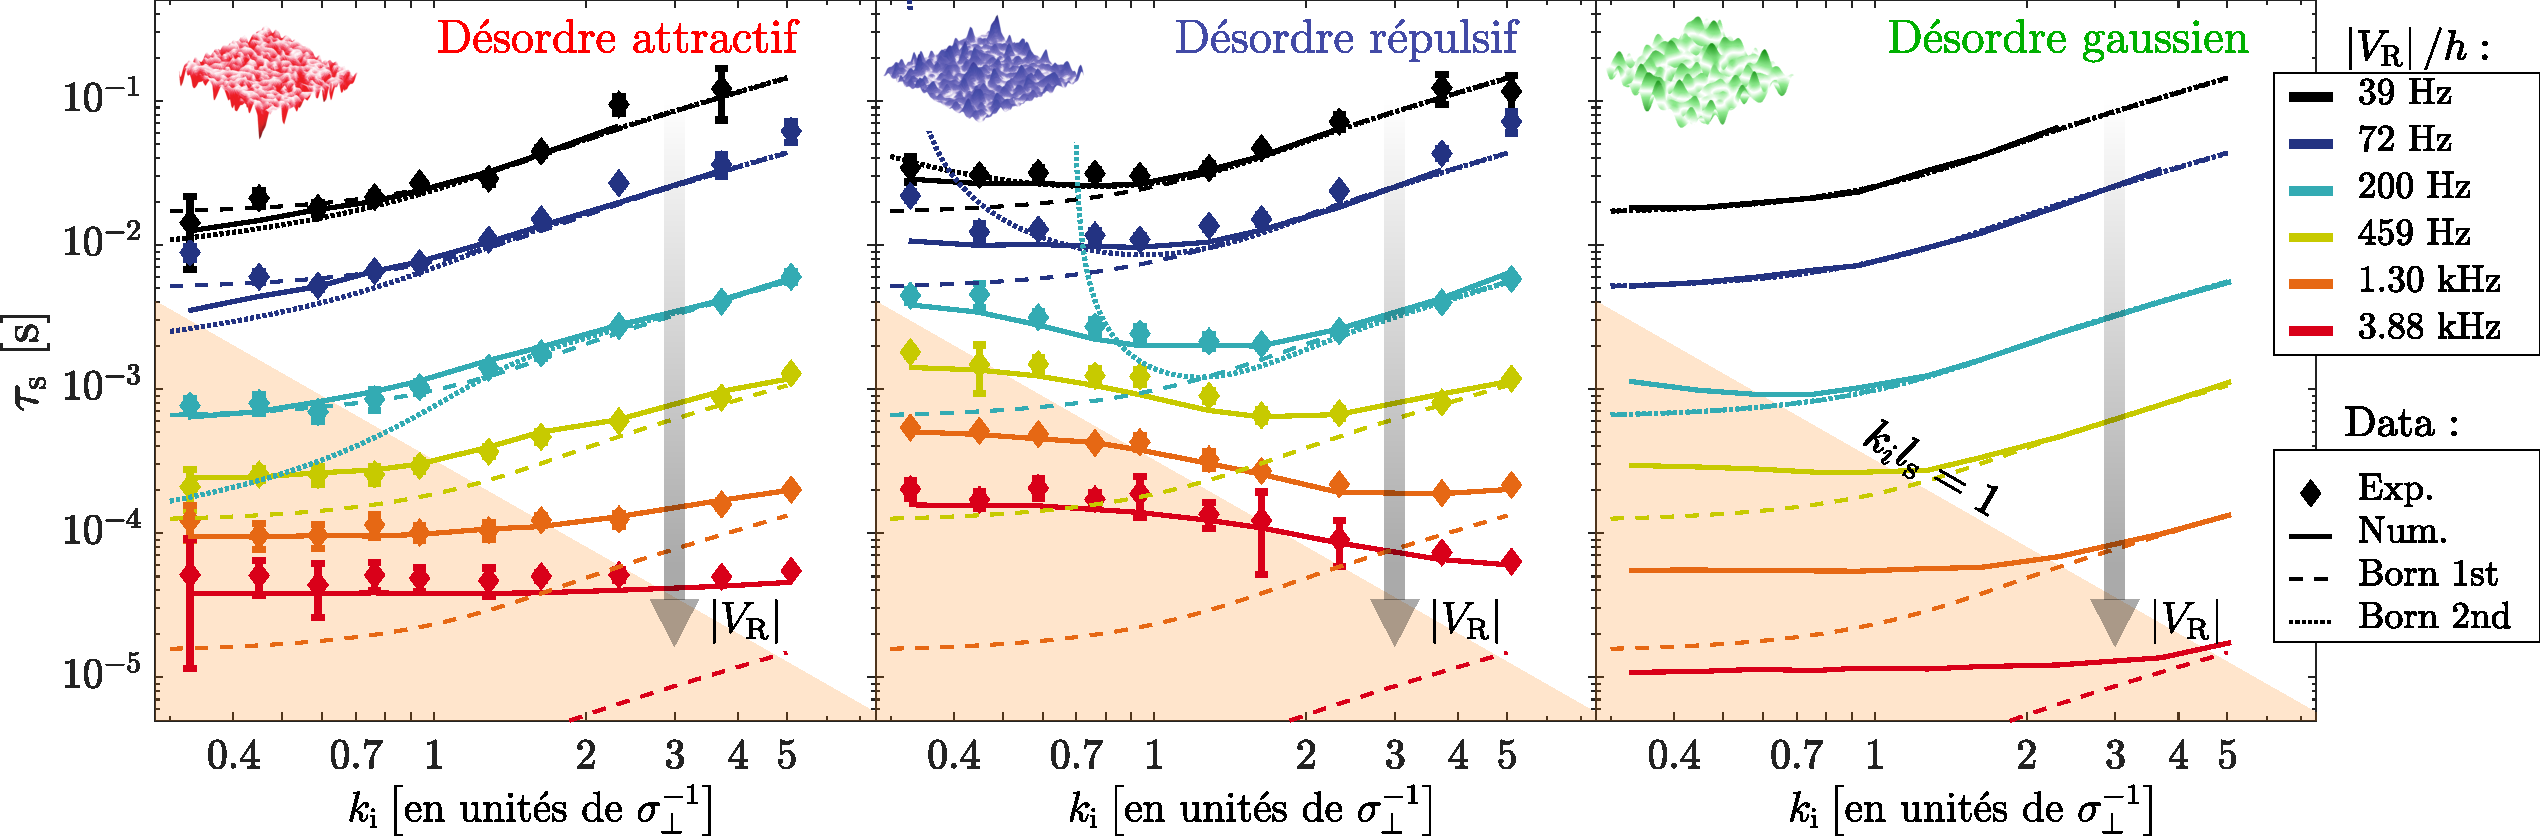
\includegraphics[width=\textwidth]{Fig/TauS_NJP/donnees_taus_ordre3.pdf}
\caption{\textbf{Données expérimentales et numériques du temps de diffusion élastique.} Les données expérimentales (points) et numériques (lignes continues) sont celles présentées dans le chapitre précédent, que nous avons complétées de simulations numériques pour un désordre gaussien. L'approximation de Born est tracée en lignes tiretées, et s'accorde sur un plan grand domaine de paramètres dans le cas d'un désordre gaussien que pour les désordres speckle. La zone orangée représente le domaine où $k_{\mathrm{i}}\ls^{\mathrm{Born}}>1$. La correction de l'approximation de Born au second ordre est représentée en lignes pointillées pour les désordres les plus faibles, et montre un accord particulièrement bon pour les désordres d'amplitude $|\VR|/h=\SI{39}{\hertz}$. L'augmentation de l'amplitude du désordre mène néanmoins à de fortes déviations vis-à-vis de nos données.}
\label{fig:donnees_taus_ordre_3}
\end{figure}

Dans le cas d'un désordre de type speckle, les corrections sont de signe opposé selon que le désordre soit attractif ($\VR^3<0$) ou répulsif ($\VR^3>0$). Dans le cas d'un désordre attractif, les corrections $-2\mathrm{Im}[\Sigma^{(2)}]$ sont positives, résultant en une diminution du temps de vie associé. Ces corrections du second ordre sont en excellent accord avec nos données dans le cas du désordre le plus faible $\VR/h=\SI{-39}{\hertz}$. En revanche, l'augmentation de l'amplitude du désordre mène à de fortes déviations, nécessitant la prise en compte d'ordres supérieurs dans la série \ref{eq:developpement_born}. 

Dans le cas d'un désordre répulsif, les corrections du second ordre sont négatives et entraînent l'augmentation de $\taus$. De même que dans le cas attractif, l'accord est remarquable pour notre désordre le plus faible, d'amplitude $\VR/h=\SI{39}{\hertz}$. Néanmoins, l'augmentation de l'amplitude du désordre rend rapidement la correction du second ordre de la self-energy comparable au premier ordre. Le temps de vie associé diverge alors, comme illustré sur la figure \ref{fig:donnees_taus_ordre_3}. Pour régulariser ce comportement, il est à nouveau nécessaire de tenir compte des ordres supérieurs. 


L'extension de l'approximation de Born à la description du régime de désordre fort demande donc la prise en compte de nombreux ordres supplémentaires. Cependant, la série \ref{eq:developpement_born} est connue pour diverger \citep{kuhn2007coherent}. Il en résulte que le développement en série de la self-energy ne permet d'étendre le régime de validité de l'approximation de Born qu'au domaine des impulsions faibles, et ne permet pas de décrire le régime de désordre fort.


\subsection{Approximation de Born auto-consistante}
Dans l'approche perturbative de Born, on peut considérer que le potentiel réalise un couplage de l'état initial $\etat{\mathbf{k}_{\mathrm{i}}}$ aux états libres $\etat{\mathbf{k}'}$ peu perturbés par le potentiel. On comprend aisément que cette considération échoue à décrire le régime de désordre fort, les états finaux $\etat{\mathbf{k}'}$ étant fortement affectés par le désordre. 

Une approche communément utilisée pour décrire le régime de désordre fort consiste à considérer que le potentiel couple l'état initial $\etat{\mathbf{}_{\mathrm{i}}}$ aux états habillés par le désordre, on parle alors d'approximation de Born auto-consistante (\emph{SCBA} pour l'anglais \emph{Self-Consistent Born Approximation}). Pour tenir compte du temps de vie et des décalages d'énergie de ces états habillés, on remplace la fonction de Green libre $G_0(E,\mathbf{k}_{\mathrm{i}})$ par la fonction de Green moyennée $\overline{G}(E,\mathbf{k}_{\mathrm{i}})$ dans l'expression du premier terme de la self-energy $\Sigma^{(1)}(E,\mathbf{k}_{\mathrm{i}})$. Le système d'équations de l'approximation auto-consistante de Born est donc
\begin{align}
\Sigma_{\mathrm{scba}}(E,\mathbf{k}_{\mathrm{i}})&=\sum_{\mathbf{k}'}{\widetilde{C}(\mathbf{k}_{\mathrm{i}}-\mathbf{k}') \overline{G}_{\mathrm{scba}}(E,\mathbf{k}')}  
\label{eq:SCBA}\\
\overline{G}_{\mathrm{scba}}(E,\mathbf{k}_{\mathrm{i}}) &= \frac{1}{E-E_{\mathrm{k}_i} - \overline{V} - \Sigma_{\mathrm{scba}}(E,\mathbf{k}_{\mathrm{i}})} \text{ ,}
\end{align}
dont la résolution se fait numériquement de manière itérative.

Il apparaît immédiatement dans le système d'équations \ref{eq:SCBA} que l'approximation auto-consistante de Born ne peut pas prédire la forme exacte des fonctions spectrales. En effet, celle-ci ne tient compte que de la fonction de corrélation à deux points du désordre, sans tenir compte de la distribution de potentiel $\mathcal{P}(V)$ \citep{pasek2015phase}. Cependant, nous allons voir que pour un désordre gaussien, celle-ci fournit une estimation convaincante de la largeur $\Delta E^{\mathrm{scba}}$ de la fonction spectrale, et donne donc une bonne estimation du temps de diffusion élastique $\taus^{\mathrm{scba}}=\hb/\Delta E^{\mathrm{scba}}$. 

Nous avons ainsi résolu le système \ref{eq:SCBA} par itérations numériques jusqu'à ce que la self-energy obtenue converge. La fonction spectrale extraite est tracée figure \ref{fig:SCBA_gauss}.a pour les paramètres $k_{\mathrm{i}}=0.93\sigmap^{-1}$ et $|\VR|/h=\lbrace \SI{39}{\hertz},\SI{458}{\hertz},\SI{3.88}{\kilo\hertz}\rbrace$. Dans le cas de désordre faible (figure en haut à gauche), la fonction spectrale obtenue par l'approximation auto-consistante de Born reproduit la forme lorentzienne attendue par l'approximation de Born au premier ordre, avec $\hb/\taus^{\mathrm{scba}}=\hb/\taus^{\mathrm{Born}}$. L'augmentation de l'amplitude du désordre $|\VR|$ montre la déviation à la forme lorentzienne attendue pour un désordre faible, et témoigne de l'élargissement de la fonction spectrale (figure en haut à droite pour un désordre d'amplitude intermédiaire $|\VR|\sim \ER$, et figure en bas à gauche pour un désordre fort $|\VR|\gg\ER$).

Il est possible de déterminer analytiquement la limite asymptotique dans le régime classique $|\VR|/\ER\rightarrow\infty$ de l'approximation auto-consistante de Born. Trappe et al. montrent ainsi que la fonction spectrale $A^{\mathrm{scba,cl}}$ est décrite par un demi-cercle de rayon $2|\VR|$ \citep{trappe2015semiclassical}
\begin{equation}
A^{\mathrm{scba,cl}}(\mathbf{k}_{\mathrm{i}},E)=\frac{1}{2\pi \VR^2} \sqrt{4\VR^2-(E-\Eki-\overline{V})^2}
\end{equation}
Dans cette limite, le temps de diffusion élastique est donné par $\taus^{\mathrm{scba,cl}}=\hb/(2\sqrt{3}|\VR|)$, indépendant de la distribution de potentiel. 

\begin{figure}
\centering
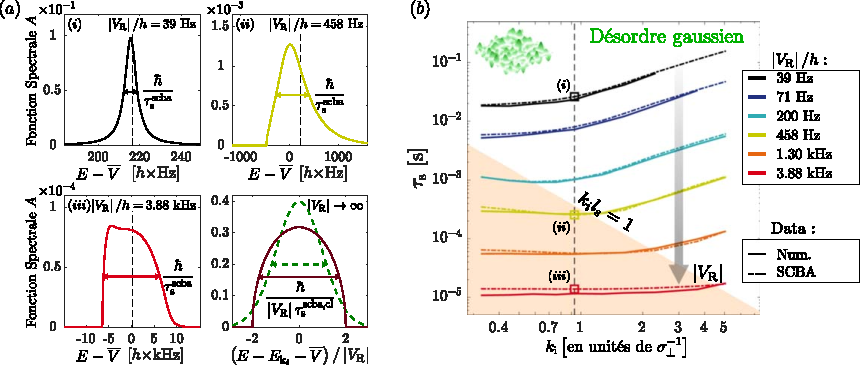
\includegraphics[width=\textwidth]{Fig/TauS_NJP/SCBA_gauss.pdf}
\caption{\textbf{Comparaison du temps de diffusion élastique d'un désordre gaussien à l'approximation auto-consistante de Born.} \textbf{a.} Exemples de fonctions spectrales obtenues en résolvant les équations de l'approximation auto-consistante de Born. Pour un désordre faible, on retrouve la forme lorentzienne attendue par l'approximation de Born au premier ordre. L'augmentation de l'amplitude du désordre se manifeste par une déviation à la forme lorentzienne et un élargissement de la fonction spectrale. Les lignes tiretées verticales indiquent la position de l'énergie cinétique. Dans la limite classique, l'approximation auto-consistante de Born prédit la forme d'un demi-cercle, tandis que la forme attendue correspond à la distribution de potentiel $\mathcal{P}(V)$, de forme gaussienne pour un désordre gaussien. \textbf{b.} Comparaison de la prédiction de l'approximation auto-consistante de Born (lignes tiretées) à nos données numériques pour un désordre gaussien (lignes continues). L'approximation auto-consistante de Born présente un accord remarquable avec nos données sur l'ensemble des paramètres, y compris au delà de la limite $k_{\mathrm{i}}\ls=1$. On remarque tout de même l'apparition de déviations pour notre désordre le plus fort $|\VR|/h=\SI{3.88}{\kilo\hertz}$.}
\label{fig:SCBA_gauss}
\end{figure}


La figure \ref{fig:SCBA_gauss}.b montre la comparaison entre nos données numériques du temps de diffusion élastique $\taus$ (lignes continues) et la prédiction de l'approximation auto-consistance de Born $\taus^{\mathrm{scba}}$ (lignes tiretées). Il apparaît alors que l'approximation auto-consistante de Born, communément utilisée en matière condensée, reproduit fidèlement nos données pour un désordre gaussien, lui aussi largement utilisé en matière condensée. L'accord en d'autant plus marquant que celui-ci s'étend au delà de la limite $k_{\mathrm{i}}\ls=1$, alors que l'approximation auto-consistante de Born ne permet pas de reproduire la forme de la fonction spectrale dans le régime classique. Néanmoins, les largeurs à mi-hauteur des fonctions spectrales sont semblables, celles-ci ne différant que d'un facteur $\sqrt{3/(2\ln 2)}\approx 1.5$, expliquant les déviations obtenues pour le désordre le plus important de $|\VR|/h=\SI{3.88}{\kilo\hertz}$.









\section{Temps de diffusion élastique et fonctions spectrales pour un désordre speckle}

Dans la section précédente, nous avons pu voir que l'extension de l'approximation de Born au deuxième ordre de la self-energy permet de décrire le régime d'impulsion faible pour des désordres faibles dans le cadre d'une théorie perturbative. Afin de décrire le régime de désordre fort, nous avons comparé la prédiction de l'approximation de auto-consistante de Born communément utilisée à nos données numériques pour un désordre gaussien, témoignant d'un bon accord sur l'ensemble de nos paramètres expérimentaux. Ces deux résultats indiquent donc que l'approche de la fonction spectrale est pertinente pour décrire la décroissance temporelle de l'état initial.

Dans cette section, nous allons décrire en quoi l'approximation auto-consistante de Born n'est pas suffisante pour décrire le régime classique dans le cas de désordres de type speckle. Nous expliquerons ensuite comment les fonctions spectrales de désordre speckle ont été mesurées expérimentalement, et nous tacherons de décrire leur comportement. Enfin, nous terminerons sur la comparaison entre les mesures du temps de diffusion élastique et le temps de vie que l'on peut extraire de la mesure des fonctions spectrales.


\subsection{Limite de l'approche auto-consistante pour un désordre de type speckle}
Si l'approximation auto-consistante de Born permet de décrire correctement l'ensemble de nos données pour un désordre gaussien, ce n'est pas le cas pour un désordre de type speckle. En effet, l'approche auto-consistante ne repose que sur la fonction de corrélation à deux corps du potentiel, et ne tient pas compte des fonctions de corrélation d'ordres supérieurs. De manière plus générale, un ingrédient essentiel manque à la description d'un désordre arbitraire: la distribution de potentiel. 

L'approche auto-consistante de Born ne contenant que des puissances paires du potentiel \citep{trappe2015semiclassical}, celle-ci ne peut pas décrire les asymétries du potentiel. L'approche auto-consistante ne peut donc pas prétendre à une meilleure description du régime de désordre faible que l'approximation de Born au second ordre pour des désordres speckle. 

La comparaison entre nos données expérimentales et la prédiction auto-consistante est montrée figures \ref{fig:comparaison_taus_specfunc_rouge} (pour un speckle attractif) et \ref{fig:comparaison_taus_specfunc_bleu} (pour un désordre répulsif). Dans le régime de désordre intermédiaire, si la comparaison de l'approximation auto-consistante s'accorde correctement aux données pour un désordre attractif, ce n'est pas le cas pour un désordre répulsif. 

Dans le régime de désordre classique, la prédiction de la \textit{SCBA} est meilleure que l'approximation de Born au premier ordre. De plus, $\taus$ et $\taus^{\mathrm{scba}}$ se comportent tous deux en $1/|\VR|$ pour un speckle attractif\footnote{Le rayon de la prédiction classique de la \textit{SCBA} et de $2|\VR|$. Dans la limite classique, la fonction spectrale converge vers la distribution de potentiel, qui correspond à une exponentielle de largeur à $1/e$ valant $|\VR|$.}, résultant en une erreur systématique d'un facteur $\taus^{\mathrm{sf,cl}}/\taus^{\mathrm{scba,cl}}\approx 5$. Expérimentalement, nous mesurons une déviation de $\taus/\taus^{\mathrm{scba,cl}}=3.2\pm0.5$, compatible avec la valeur théorique\footnote{Cette valeur provient de la valeur de $\taus$ mesurée pour notre désordre le plus fort $|\VR|/\ER\sim 8.5$ et d'impulsion $k_{\mathrm{i}}=0.33\sigmap^{-1}$. Pour ces paramètres, le régime classique n'est pas encore entièrement atteint, voir \citep{prat2016semiclassical} par exemple.}. 

Dans le cas d'un désordre répulsif, l'accord est bien moins correct et l'approximation auto-consistante échoue à décrire les données expérimentales. Cet effet montre clairement le manquement de la \textit{SCBA} à décrire le régime classique pour lequel la distribution de potentiel est capitale. Il apparaît donc nécessaire d'analyser les détails de la fonction spectrale pour un désordre de type speckle.







\subsection{Fonctions spectrales d'un désordre speckle}
Nous avons pu voir au cours du chapitre \ref{ch:Localisation} l'importance de la détermination précise des fonctions spectrales. Cette idée n'en a été que renforcée par l'étude détaillée du comportement du temps de diffusion élastique. Dans la perspective d'adresser spécifiquement les niveaux d'énergie du désordre, l'équipe a mis en place un chargement spectroscopique du désordre, permettant la détermination expérimentale des fonctions spectrales pour un désordre de type speckle. Ces mesures ont fait l'objet de la thèse de Vincent Denechaud, où de nombreux détails expérimentaux et théoriques pourront être retrouvés \citep{denechaud2018vers}.


\paragraph*{Mesure des fonctions spectrales}
Le protocole de mesure des fonctions spectrales est schématisé sur la figure \ref{fig:illustration_fonction_spectrale}. Celui-ci combine de nombreuses astuces expérimentales que nous avons présentées dans les chapitres précédents, notamment l'approche de désordre dépendant de l'état interne (voir section \ref{sc:state_dependent_disorder}), et l'utilisation d'un champ magnétique magique (voir section \ref{sc:implementation_levitation}). 

L'utilisation de l'approche de potentiel dépendant de l'état interne nécessite d'utiliser un sous-état Zeeman dans chacun des états hyperfins $\etatF{1}{}$ et $\etatF{2}{}$. On note ainsi les états correspondants $\etat{1}=\etatF{1}{-1}$ et $\etat{2}=\etatF{2}{+1}$, pour lesquels il existe un biais magnétique \emph{magique} $\magicB=\SI{3.2}{\gauss}$ où les états $\etat{1}$ et $\etat{2}$ possèdent la même susceptibilité magnétique. Le choix de ces états permet donc d'affranchir la séparation en énergie de ces niveaux des fluctuations de champ magnétique en plus d'être lévités simultanément.

Le chargement du désordre à une énergie bien définie nécessite de coupler les états $\etat{1}$ $\etat{2}$ afin de pouvoir transférer les atomes initialement dans l'état libre vers l'état habillé par le désordre. Compte-tenu de la séparation entre ces états, le choix d'un transfert radio-fréquences est retenu, appuyé par l'excellent contrôle des fréquences qu'il est possible d'obtenir. En raison de la séparation en spin de $\Delta\mf=2$, il s'agira donc d'une transition à deux photons.




\begin{figure}
\centering
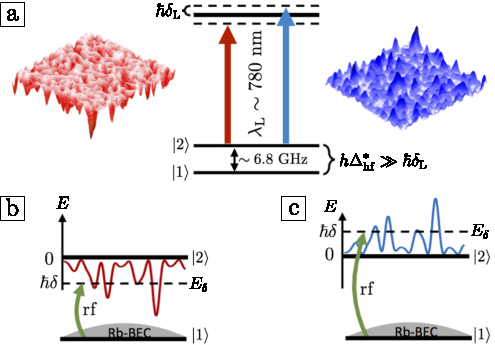
\includegraphics[scale=1.2]{Fig/TauS_NJP/illustration_mesure_fonction_spectrale.pdf}
\caption{\textbf{Illustration du protocole spectroscopique de mesure des fonctions spectrales.} \textbf{a.} Illustration du protocole de génération de speckle dépendant de l'état interne. Un laser quasi-résonant sur l'état $\protect\etat{2}$ génère un potentiel attractif (pour $\delta_{\mathrm{L}}<0$) ou bien répulsif (pour $\delta_{\mathrm{L}}>0$). Ce potentiel qui est négligeable pour l'état $\protect\etat{1}$ en raison du grand désaccord $2\pi\deltahf^*+\delta_{\mathrm{L}}$ lié à la séparation hyperfine. \textbf{b. et c.} Illustration du protocole de spectroscopie. L'état $\protect\etat{1}$ libre est transféré vers l'état $\protect\etat{2}$ habillé par le désordre à l'aide de radio-fréquences. Le choix d'un désaccord $\delta$ par rapport à la résonance $\protect\etat{1}\rightarrow \protect\etat{2}$ en absence de désordre permet d'adresser une énergie bien définie dans le désordre. }
\label{fig:illustration_fonction_spectrale}
\end{figure}

La séquence commence par la création d'un condensat de Bose-Einstein  très décomprimé d'environ \SI{2e5}{} atomes de \isotope[87]{Rb} dans l'état $\etat{1}$. Le désordre est allumé brusquement à $t=0$, et simultanément  le transfert radio-fréquences a lieu pendant une durée $t_0$. Le taux de transfert est ensuite mesuré en imageant par fluorescence sélectivement les atomes dans l'état $\etat{2}$
\begin{equation}
n_2(t_0)=n_1(0) \times \Gamma t_0 \text{ .}
\end{equation}



Les atomes transférés possèdent une énergie finale $E_{\mathrm{f}}=E_{\mathrm{i}} +\hb\omega$, avec $\omega$ la pulsation de la radio-fréquence rayonnée. Il est possible d'assimiler l'état initial à une onde plane d'impulsion nulle $\etat{\mathbf{k}=0}$ dans la mesure où $\mu\ll\VR$, et son énergie $E_{\mathrm{i}}$ correspond alors à l'énergie interne $E_{\etat{1}}$. On montre alors que les atomes transférés dans le désordre possèdent une énergie externe $E=\hb\delta$, où $\delta=\omega-2\pi \deltahf^*$ correspond au désaccord par rapport à la résonance au biais magique en absence de désordre donnée par $\deltahf^*=E_{\etat{2}}-E_{\etat{1}}\approx \SI{6.8}{\giga\hertz}$, c'est à dire la différence d'énergie interne. Cette situation est schématisée dans la partie basse de la figure \ref{fig:illustration_fonction_spectrale}. Étant donné le temps fini de transfert radio-fréquence, l'énergie adressée dans le désordre possède une résolution $\Delta E\sim \hb/t_0$ mesurée à l'aide d'un spectre de Rabi à deux photons en absence de désordre. Il a ainsi été montré que pour un temps de transfert de \SI{100}{\milli\second}, la résolution en énergie obtenue était d'environ $h\times\SI{10}{\hertz}$, correspondant à la limite de Fourier\footnote{Nous avons récemment pu obtenir une résolution de $h\times\SI{5}{\hertz}$ grâce à l'étude détaillée des champs magnétiques dans la chambre de science.}. 









\paragraph*{Correspondance entre fonction spectrale et taux de transfert}
Nous avons vu dans le paragraphe précédent comment nous pouvons mesurer le taux de transfert des atomes dans le désordre à une énergie ciblée. Celui-ci est relié à la fonction spectrale $A(\mathbf{k}=0,E)$, que nous pouvons réécrire
\begin{align}
A(\mathbf{k}=0,E)&=\overline{\left\langle \mathbf{k}=0 \left| \delta(E-\hat{H}) \right| \mathbf{k}=0 \right\rangle} \\
&= \overline{\sum_{\alpha}{|\langle\mathbf{k}=0 | \psi_{\alpha}\rangle|^2.\delta(E-E_{\alpha})}}
\end{align}
en introduisant les états propres $\etat{\psi_{\alpha}}$ du désordre et d'énergie $E_{\alpha}$. Les fluctuations du terme de recouvrement $|\langle \mathbf{k}=0 | \psi_{\alpha} \rangle|^2$ disparaissent avec le moyennage sur les différentes réalisations du désordre. On peut alors sortir sa valeur moyenne $\overline{|\langle \mathbf{k}=0 | \psi_{\mathrm{E}} \rangle|^2}$ à l'énergie $E$ de la somme:
\begin{align}
A(\mathbf{k}=0,E)&\approx \overline{|\langle \mathbf{k}=0 | \psi_{\alpha} \rangle|^2}. \overline{\sum_{\alpha}{\delta(E-E_{\alpha})}} \\
&\approx \overline{|\langle \mathbf{k}=0 | \psi_{\mathrm{E}} \rangle|^2} . \rho(E) \text{ .}
\end{align}
La fonction spectrale apparaît alors comme correspondant au recouvrement moyen entre l'état initial et les états d'énergie $E$ du désordre.

Cette dernière expression présente un intérêt expérimental particulier. En effet, on peut montrer à l'aide de la règle d'or de Fermi que
\begin{equation}
\Gamma(\delta)=2 \pi \hb \Omega^2 \overline{|\langle \psi_{\delta} | \mathbf{k}=0 \rangle|^2} . \rho(\hb\delta) \propto A(\mathbf{k}=0 ,\hb \delta) \text{ ,}
\end{equation}
où $\Gamma(\delta)$ correspond au taux de transfert entre l'état initial du condensat de Bose-Einstein $\etat{\mathbf{k}=0}$ et les états $\etat{\psi_{\delta}}$ d'énergie externe $E=\hb\delta$ du désordre réalisé à l'aide d'un couplage de pulsation de Rabi $\Omega$. La mesure de la fonction spectrale peut donc être faite en déterminant le taux de transfert d'une spectroscopie du désordre.

De nombreuses hypothèses sont nécessaires pour obtenir ce résultat, dont une discussion détaillée est donnée dans les références \citep{denechaud2018vers}\citep{volchkov2018measurement}. Notamment, cette correspondance entre fonction spectrale et taux de transfert n'est valide que pour un couplage faible ($\Omega$ petit devant les autres échelles d'énergie) et des temps $t$ courts tels que $\Gamma t \ll 1$. Une conséquence forte de ces contraintes est seuls quelques pourcents des atomes sont transférés dans le désordre. 



\paragraph*{Résultats}
L'ensemble des mesures des fonctions spectrales $A(\mathbf{k}=0,E=\hb\delta)$ est représenté figures \ref{fig:mesures_fonctions_spectrales_rouge} et \ref{fig:mesures_fonctions_spectrales_bleu} en points bleus. Sur ces mêmes figures sont tracées en rouge des simulations numériques réalisées par Michael Pasek et Dominique Delande du Laboratoire Kastler Brossel, dont les détails peuvent être retrouvés dans la référence \citep{volchkov2018measurement}. Afin de comparer les données expérimentales et les simulations, l'amplitude du désordre expérimental est calibrée à l'aide de la fonction spectrale numérique pour $\VR/h=\SI{-121}{\hertz}$, permettant de corriger la mesure photométrique de l'amplitude du désordre. 

L'accord entre les données expérimentales et numériques est remarquable: les données expérimentales se superposent aux simulations sur l'ensemble des paramètres expérimentaux, sans paramètre ajustable. De plus, chaque point correspond à un unique cycle expérimental: il n'y a pas de moyennage sur les réalisations du désordre pour les données expérimentales. La validation de l'hypothèse ergodique repose notamment sur le fait que notre condensat de Bose-Einstein est très grand devant la taille des grains du désordre\footnote{Le rayon de Thomas-Fermi de notre condensat est d'environ \SI{30}{\micro\metre}, bien plus grand que les tailles des grains de speckle $\sigmap=\SI{0.5}{\micro\metre}$ et $\sigmal\approx\SI{4.1}{\micro\metre}$.}, chaque atome ressentant une réalisation du désordre différente.


Deux régimes se distinguent.

régime quantique, régime classique
résonance du bleu



\begin{figure}
\centering
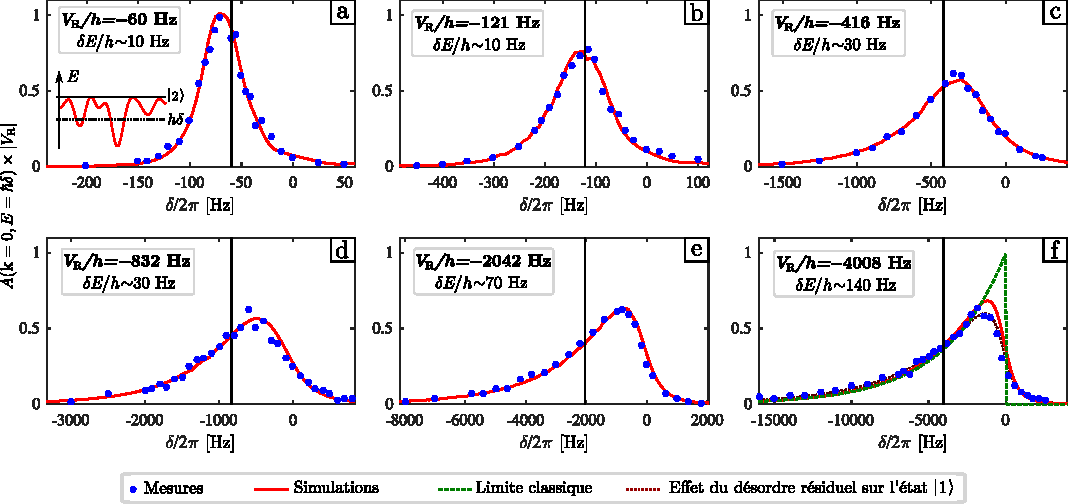
\includegraphics[width=\textwidth]{Fig/TauS_NJP/fonctions_spectrales_rouge.pdf}
\caption{\textbf{Mesures des fonctions spectrales pour un désordre attractif.} Stuff.}
\label{fig:mesures_fonctions_spectrales_rouge}

\vspace{1cm}
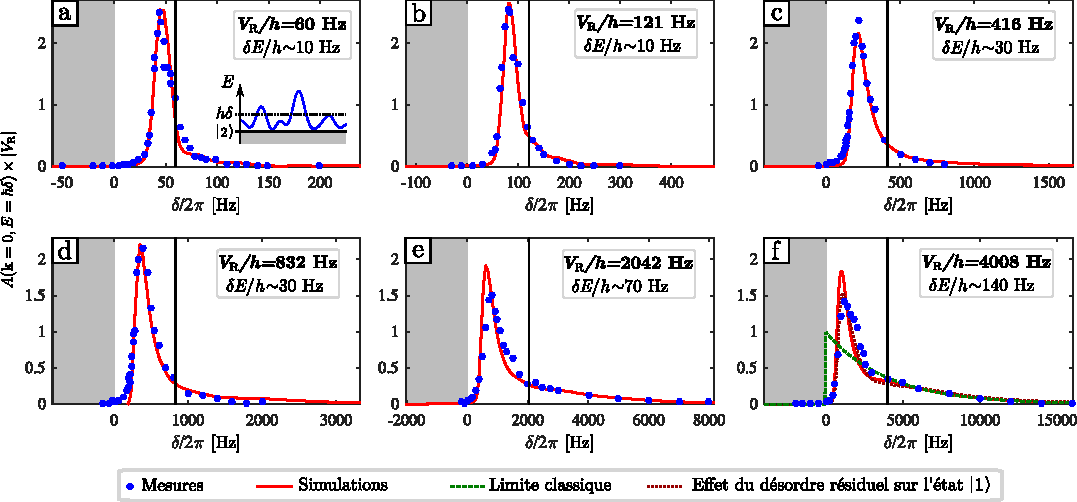
\includegraphics[width=\textwidth]{Fig/TauS_NJP/fonctions_spectrales_bleu.pdf}
\caption{\textbf{Mesure des fonctions spectrales pour un désordre répulsif.} Stuff.}
\label{fig:mesures_fonctions_spectrales_bleu}
\end{figure}





\subsection{Comparaison du temps de diffusion élastique avec les fonctions spectrales mesurées}
Comme nous avons vu précédemment, il est possible de donner une estimation du temps de vie de l'état initial $\etat{\mathbf{k}_{\mathrm{i}}}$ dans le désordre à l'aide de la largeur à mi-hauteur de la fonction spectrale. Nous pouvons alors extraire un temps $\taus^{\mathrm{sf}}$ des fonctions spectrales mesurées $A(\mathbf{k}=0,E)$ mesurées pour différentes amplitudes de désordre $\VR$.

Dans le cas d'un désordre attractif, la largeur à mi-hauteur de la fonction spectrale mesurée est obtenue à l'aide d'un ajustement des données expérimentales par la convolution d'une lorentzienne avec une fonction exponentielle \ref{eq:distribution_potentiel_speckle}, qui permet de reproduire fidèlement  la forme de fonctions spectrales pour toutes les amplitudes de désordre. La largeur à mi-hauteur $\Delta E$ est ensuite extraite à l'aide d'un algorithme, permettant de déterminer un temps de vie $\taus^{\mathrm{sf}}=\hb/\Delta E$ pour chaque amplitude de désordre considérée. Le temps de vie pour n'importe quelle amplitude de désordre est ensuite obtenue par interpolation.

Les valeurs de $\taus^{\mathrm{sf}}$ sont donc déterminées pour les amplitudes de désordres considérées  dans le chapitre \ref{ch:TauS_PRL}. Celles-ci sont tracées aux côtés des mesures de $\taus$ dans la figure \ref{fig:comparaison_taus_specfunc_rouge} et montrent un bon accord avec les mesures à impulsion faible, notamment dans le domaine de désordre fort. Cet accord entre données temporelles et données dans le domaine des énergies indique que nos mesures de $\taus$ sont entièrement compatibles avec le profil des fonctions spectrales pour un désordre speckle attractif.


\begin{figure}
\centering
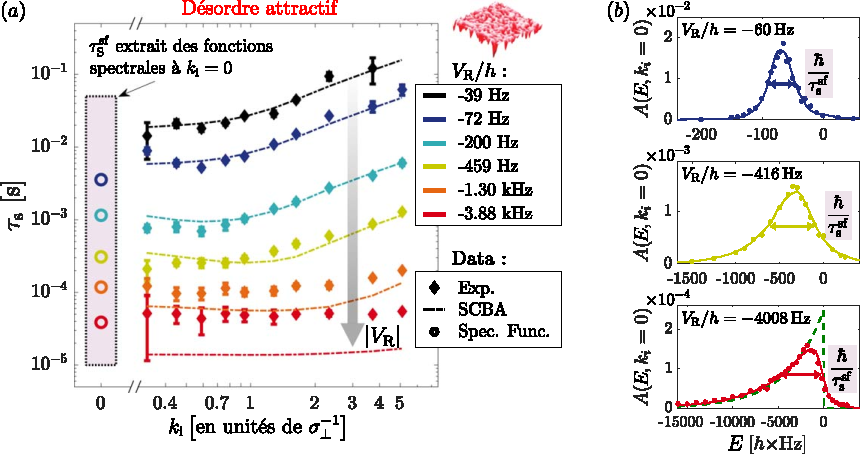
\includegraphics[width=\textwidth]{Fig/TauS_NJP/comparaison_specfunc_taus_rouge.pdf}
\caption{\textbf{Comparaison des fonctions spectrales mesurées au temps de diffusion élastique pour un speckle attractif.} \textbf{a.} Le temps de diffusion élastique est comparé à la prédiction de l'approximation auto-consistante de Born. Cette dernière est proche des données expérimentales dans le régime de désordre faible, mais ne permet pas de décrire le régime de désordre fort. La \textit{SCBA} échoue de plus à décrire les asymétries du potentiel. Les temps de vie $\taus^{\mathrm{sf}}$ extraits des fonctions spectrales mesurées sont compatibles avec les mesures de $\taus$ de basse impulsion.\textbf{b.} Illustration de l'extraction du temps de vie $\taus^{\mathrm{sf}}$. Le temps de vie est extrait en déterminant la largeur à mi-hauteur d'une fonction d'ajustement des données expérimentales. Ces données sont celles de la figure \ref{fig:mesures_fonctions_spectrales_rouge}.}
\label{fig:comparaison_taus_specfunc_rouge}
\end{figure}


Comme nous avons vu dans la section précédente, un désordre speckle répulsif présente un comportement pathologique en raison de la présence d'une résonance sur les premiers états liées du désordre. Cette pathologie se manifeste sous la forme d'un pic de résonance dans la fonction spectrale. On s'attend alors à ce que l'évolution temporelle de l'état initial présente deux échelles de temps différentes en raison de la double structure de la fonction spectrale. Un premier temps court est associé à la structure large de la distribution de potentiel, tandis qu'un second temps, plus long, est dû à la structure étroite de la résonance à basse énergie. Expérimentalement, nous ne sommes sensibles qu'à ce dernier temps.

Comme précédemment, le temps de vie estimé de l'état initial est obtenu en déterminant la largeur de la fonction spectrale mesurée expérimentalement par un ajustement. Afin de tenir compte de la double structure, la fonction heuristique d'ajustement est donnée par la somme de la convolution d'une lorentzienne et d'une exponentielle \ref{eq:distribution_potentiel_speckle}, comme précédemment, et d'une gaussienne étroite pour décrire le pic de résonance. On reproduit ainsi la forme des fonctions spectrales mesurées de manière fidèle. Le temps de vie $\taus^{\mathrm{sf}}$ est extrait de la largeur à mi-hauteur de cette gaussienne, et une interpolation permet de l'estimer pour différentes amplitudes de désordre. 

Ces mesures de $\taus^{\mathrm{sf}}$ sont confrontées aux mesures de $\taus$ sur la figure \ref{fig:comparaison_taus_specfunc_bleu} et témoignent d'un très bon accord avec les données à basse impulsion, particulièrement dans le régime classique. De même que pour un speckle attractif, cette comparaison entre données temporelles et données spectrales montre qu'il est capital de connaître précisément les détails de la fonction spectrale pour étudier la dynamique de l'état initial.

\begin{figure}
\centering
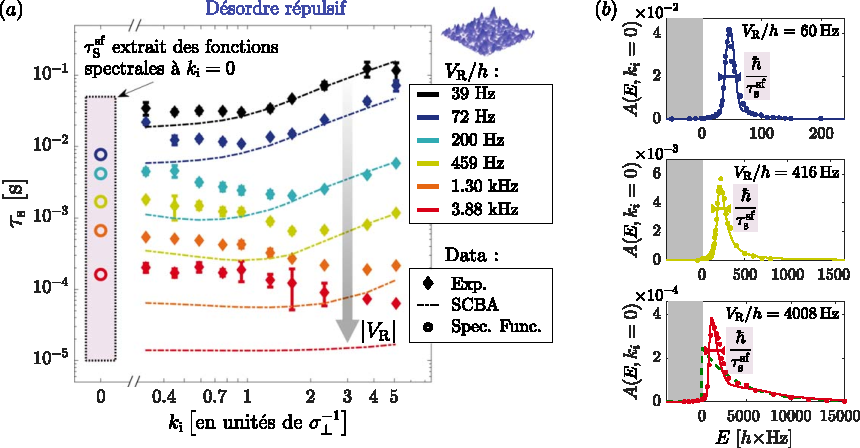
\includegraphics[width=\textwidth]{Fig/TauS_NJP/comparaison_specfunc_taus_bleu.pdf}
\caption{\textbf{Comparaion des fonctions spectrales mesurées au temps de diffusion élastique pour un speckle répulsif.} \textbf{a.} Les données expérimentales du temps de diffusion élastique sont comparées à la prédiction de l'approximation auto-consistante de Born. Celle-ci ne permet de rendre compte que du régime de désordre faible, et de grande impulsion, et échoue encre à décrire les asymétries du potentiel. Les temps de vie $\taus^{\mathrm{sf}}$ estimés à partir du pic de résonance des fonctions spectrales mesurées sont tout à fait compatibles avec les mesures du temps de diffusion élastique à faible impulsion. \textbf{b.} Illustration de l'extraction du temps de vie $\taus^{\mathrm{sf}}$. Le temps de vie est extrait en déterminant la largeur à mi-hauteur d'une fonction d'ajustement bi-modale des données expérimentales. Plus particulièrement, le temps de vie est extrait de la largeur à mi-hauteur de la structure étroite associée à la résonance des premiers états liés du désordre. Ces données sont celles de la figure \ref{fig:mesures_fonctions_spectrales_bleu}.}
\label{fig:comparaison_taus_specfunc_bleu}
\end{figure}


